%%%%%%%%%%%%%%%%%%%%%%%%%%%%%%%%%%%%%%%%%%%%%%%%%%%%%%%%%%%%%%%%%%%%%%%%%%
%% European Journal of Operational Research --- Supplementary Materials
%% (resubmission version). Built from supplementary_trsc.tex (TS-2026-0253
%% desk-rejected; body is current as of v2.4.6). Original supplementary.tex
%% retained unchanged for history.
%%%%%%%%%%%%%%%%%%%%%%%%%%%%%%%%%%%%%%%%%%%%%%%%%%%%%%%%%%%%%%%%%%%%%%%%%%

\documentclass[11pt]{article}
\usepackage[margin=1in]{geometry}
\usepackage{amsmath,amssymb,amsthm}
\usepackage{mathtools}
\usepackage{graphicx}
\usepackage{booktabs}
\usepackage{multirow}
\usepackage{natbib}
\usepackage{hyperref}
\usepackage{enumitem}
\usepackage{xcolor}
\usepackage[affil-it]{authblk}
\usepackage{setspace}
\usepackage{caption}
\usepackage{xr}
\externaldocument{main_ejor}
\onehalfspacing

\captionsetup[table]{skip=8pt}
\hypersetup{colorlinks=true, linkcolor=blue!50!black, citecolor=blue!50!black, urlcolor=blue!60!black}

\graphicspath{{../figures/}{../code/figures/}}

% S-prefix on section, figure, and table numbers (EJOR e-companion convention).
\renewcommand{\thesection}{S\arabic{section}}
\renewcommand{\thefigure}{S\arabic{figure}}
\renewcommand{\thetable}{S\arabic{table}}

\newcommand{\F}{\mathcal{F}}
\newcommand{\Fp}{\mathcal{F}^{\mathrm{p}}}
\newcommand{\N}{N}
\newcommand{\CW}{\mathrm{CW}}
\newcommand{\cstar}{c^{\ast}}

\theoremstyle{plain}
\newtheorem{theorem}{Theorem}
\newtheorem{lemma}[theorem]{Lemma}
\newtheorem{corollary}[theorem]{Corollary}
\newtheorem{proposition}[theorem]{Proposition}

\theoremstyle{definition}
\newtheorem{definition}[theorem]{Definition}
\newtheorem{example}[theorem]{Example}

\theoremstyle{remark}
\newtheorem{remark}[theorem]{Remark}

\title{\textbf{Supplementary Materials for:\\
Online Traveling Salesman Games: Core Fragility and the Temporal Nucleolus under Dynamic Arrivals}}

\author[1]{Seyun Jeong\thanks{\texttt{jeongsseyyun@kitech.re.kr}}}
\author[1]{Hyunchul Tae\thanks{Corresponding author. \texttt{sage@kitech.re.kr}}}
\affil[1]{Korea Institute of Industrial Technology (KITECH), Cheonan, Republic of Korea}

\date{May 7, 2026}

\begin{document}
\maketitle

\section*{Electronic Companion}

\section*{Overview}
This document provides supplementary material for the above manuscript. \S\ref{app:aux} breaks down the aggregate Core-existence rates of the main manuscript's Section~6.4 by arrival pattern and coalition size. \S\ref{app:scale-invariance} documents the empirical verification of the dimensionless joint-rescaling invariance declared in the main manuscript's Section~6.1. \S\ref{app:restricted-lp} details the restricted Core LP methodology used for scale-up instances where $2^n-1$ enumeration is infeasible, together with the full binding-size distributions for the 10 near-complement and 9 intermediate-coalition main-grid cases under nearest-neighbor (NN) dispatch, and includes a note on the Temporal Nucleolus cascade implementation. \S\ref{app:open-problem} reports the empirical coverage audit of the balanced-near-complement threshold (Corollary~\ref{cor:balanced-near-complement}) on the 10 near-complement main-grid instances. \S\ref{secS:robustness-detail} reports the per-policy robustness analysis under nearest-neighbor (NN), cheapest-insertion (CI), and batch re-optimization (BR) dispatch over the 175-instance grid in full detail, including Table~\ref{tab:policy} and the empty-mechanism breakdown summarized in Section~\ref{ssec:policy} of the main manuscript. \S\ref{app:example-reduction} works out the Solomon~C101 illustrative example, states and proves the reduction of the Online~TSG to the static game at simultaneous arrivals, and reports its numerical verification on 25 pattern-A instances. \S\ref{app:inheritance} states and proves the inheritance of static Core stability under exact online dispatch. \S\ref{app:complement-feasibility-lemmas} records two auxiliary feasibility lemmas (Lemmas~\ref{lem:lemma51} and~\ref{lem:lemma52}) lifted from the main manuscript for compactness. \S\ref{app:partition-pair-cases} reports the partition-pair certificates for the 9 intermediate-coalition cases of Observation~\ref{obs:intermediate}, supporting Theorem~\ref{thm:partition-pair}. \S\ref{app:sharpness} contains the threshold-distribution histograms for $r^{\ast\ast}$, $r^{\ast\ast\ast}$, and $r^{\ast}$. Cross-document references to Theorems, Propositions, Corollaries, Remarks, Observations, Sections, Figures, and Tables resolve via the \texttt{xr} package: numbers without prefix refer to the main manuscript; supplementary objects are cited as ``Supplementary Proposition~S$x$,'' etc., or by section anchor.

\section{Per-pattern Core-existence breakdown}
\label{app:aux}

Figure~\ref{fig:core-n} breaks down the aggregate Core-existence rates of Section~6.4 of the main manuscript by arrival pattern and coalition size $n$ under nearest-neighbor (NN) dispatch. Two patterns retain $100\%$ Core existence across all $n\in\{5,7,10,12,15\}$: light-load sequential $\text{B}_{\text{light}}$ ($\rho=0.5$) and reverse-zig-zag D ($\rho=1$). Pattern E ($\rho=1$, random) holds at $100\%$ for $n\in\{5,7,15\}$ and dips to $80\%$ at $n\in\{10,12\}$ via the intermediate-coalition mechanism of Observation~\ref{obs:intermediate}. Pattern $\text{B}_{\text{medium}}$ fluctuates between $40\%$ and $80\%$ ($n=5{:}80\%$, $n=7{:}40\%$, $n=10{:}40\%$, $n=12{:}40\%$, $n=15{:}80\%$), again driven by intermediate-coalition empties at $k<n-1$. Heavy-load $\text{B}_{\text{heavy}}$ ($\rho=4$) and clustered C ($\rho=2$) are Core-fragile across the grid: $\text{B}_{\text{heavy}}$ shows $60\%$, $20\%$, $0\%$, $0\%$, $20\%$ as $n$ increases, while C shows $40\%$, $60\%$, $20\%$, $20\%$, $0\%$. Simultaneous arrivals (A) collapse non-monotonically from $60\%$ at $n\in\{5,7\}$ to $20\%$, $40\%$, and finally $0\%$ at $n=15$. Figure~\ref{fig:core-k} of the main manuscript summarizes this by peak-queue regime $k$, showing how $k=n$ (saturated) drives most empty Cores while $k<n-1$ (shallow queue) preserves Core existence except for the intermediate-coalition cases in $\text{B}_{\text{medium}}$ and E.

\begin{figure}[h]
\centering
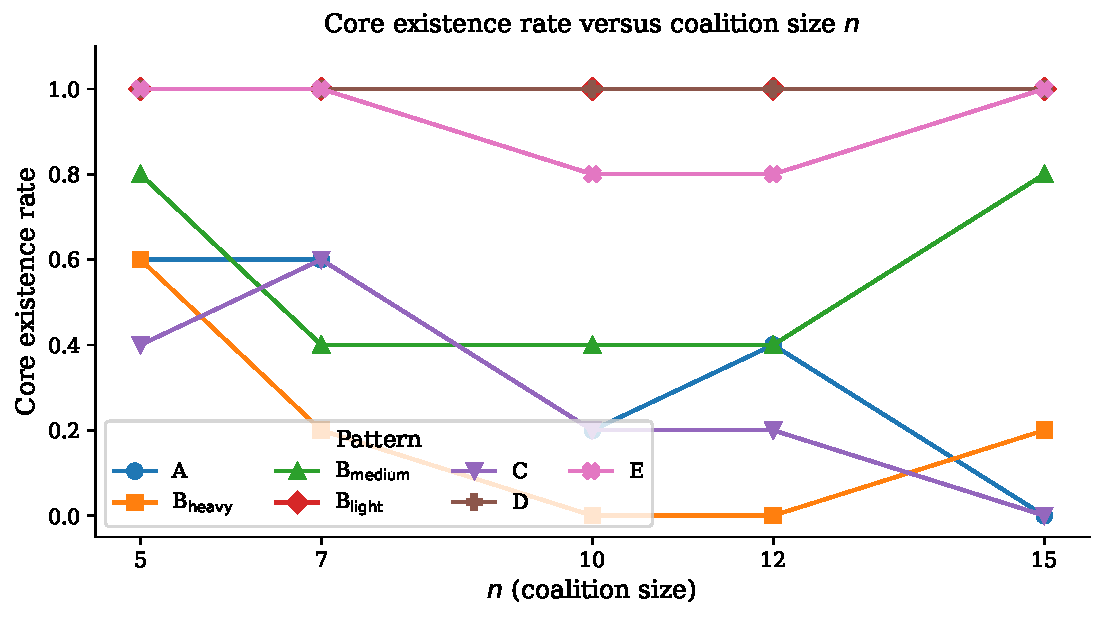
\includegraphics[width=0.75\textwidth]{fig3_core_vs_n.pdf}
\caption{Core-existence rate versus coalition size $n$, broken down by arrival pattern. Patterns $\text{B}_{\text{light}}$ and D overlap at $1.00$ across the grid. Pattern E holds at $1.00$ except at $n\in\{10,12\}$ where it dips to $0.80$. $\text{B}_{\text{medium}}$ fluctuates between $0.40$ and $0.80$. $\text{B}_{\text{heavy}}$ varies non-monotonically ($0.60$, $0.20$, $0$, $0$, $0.20$) as $n$ grows, while clustered C declines from $0.60$ to $0$ across the grid. Simultaneous arrivals (A) collapse non-monotonically to $0\%$ at $n=15$. Per-cell rates rest on five replicates, so per-cell Wilson 95\% CIs are wide ($\approx \pm 30$--$40$ percentage points; e.g., the $4/5=0.80$ rate has CI $[0.38, 0.96]$ and the $3/5=0.60$ rate has CI $[0.23, 0.88]$); within-pattern rate trends should be read accordingly.}
\label{fig:core-n}
\end{figure}

\section{Scale invariance: empirical verification}
\label{app:scale-invariance}

This section verifies empirically the scale invariance stated in Section~6.1 of the main manuscript: that all dimensionless observables are invariant under the joint rescaling $(L, v, \tau) \to (\alpha L, \alpha v, \alpha \tau)$ for any $\alpha > 0$. Since we fix $v = 1$ throughout, this reduces to the simultaneous scaling $(L, \tau) \to (\alpha L, \alpha \tau)$ with the ratio $L/\tau$ (hence the load parameter $\rho$) preserved.

\paragraph{Experimental setup.} Fixing seed $=42$, we generate instances at $n\in\{10,20\}$ and patterns $\{\text{B}_{\text{heavy}},\text{B}_{\text{medium}}, C\}$ under four scale factors $\alpha\in\{0.5,1.0,2.0,5.0\}$. For each configuration, coordinates are sampled from $[0,\alpha\sqrt{n}]^2$ and arrival intervals are scaled from the pattern-prescribed base $\tau_0=\beta_{\mathrm{BHH}}/\rho$ to $\alpha\tau_0$. The nearest-neighbor dispatch policy runs on all 24 instances. Statistics $r$, $r^{\ast\ast}$, and $k$ are recorded.

\paragraph{Results.} Table~\ref{tab:scale-invariance} reports the full 24 instances. For each of the six $(n,\text{pattern})$ configurations, all four $\alpha$ values yield \emph{bit-identical} statistics: the relative standard deviation of $r$ across $\alpha$ is $0$ to machine precision, and $k$ and $r^{\ast\ast}$ are unchanged across $\alpha$ in every configuration. Only the dimensional quantities $L$ and $\tau$ scale linearly with $\alpha$ as expected.

\begin{table}[htbp]
\centering
\footnotesize
\caption{Scale invariance verification (NN policy, seed $=42$). Each row corresponds to one $(n,\text{pattern},\alpha)$ configuration; 24 rows total. Within each $(n,\text{pattern})$ block, the four $\alpha$ values yield identical $r$, $r^{\ast\ast}$, and $k$, confirming joint-rescaling invariance to machine precision. Em-dashes in $r^{\ast\ast}$ indicate configurations where the single-complement threshold of the main manuscript's Corollary~\ref{cor:single-complement} is inapplicable (no complement coalition feasible).}
\label{tab:scale-invariance}
\begin{tabular}{@{}cccccccc@{}}
\toprule
$n$ & Pattern & $\alpha$ & $L$ & $\tau$ & $r$ & $r^{\ast\ast}$ & $k$ \\
\midrule
10 & $\text{B}_{\text{heavy}}$ & 0.5 & 1.5811 & 0.0891 & 1.4225 & 1.1324 & 10 \\
10 & $\text{B}_{\text{heavy}}$ & 1.0 & 3.1623 & 0.1781 & 1.4225 & 1.1324 & 10 \\
10 & $\text{B}_{\text{heavy}}$ & 2.0 & 6.3246 & 0.3562 & 1.4225 & 1.1324 & 10 \\
10 & $\text{B}_{\text{heavy}}$ & 5.0 & 15.8114 & 0.8905 & 1.4225 & 1.1324 & 10 \\
\midrule
10 & $\text{B}_{\text{medium}}$ & 0.5 & 1.5811 & 0.1781 & 1.4225 & 1.1324 & 10 \\
10 & $\text{B}_{\text{medium}}$ & 1.0 & 3.1623 & 0.3562 & 1.4225 & 1.1324 & 10 \\
10 & $\text{B}_{\text{medium}}$ & 2.0 & 6.3246 & 0.7124 & 1.4225 & 1.1324 & 10 \\
10 & $\text{B}_{\text{medium}}$ & 5.0 & 15.8114 & 1.7810 & 1.4225 & 1.1324 & 10 \\
\midrule
10 & C & 0.5 & 1.5811 & 0.1781 & 1.2531 & 1.1324 & 10 \\
10 & C & 1.0 & 3.1623 & 0.3562 & 1.2531 & 1.1324 & 10 \\
10 & C & 2.0 & 6.3246 & 0.7124 & 1.2531 & 1.1324 & 10 \\
10 & C & 5.0 & 15.8114 & 1.7810 & 1.2531 & 1.1324 & 10 \\
\midrule
20 & $\text{B}_{\text{heavy}}$ & 0.5 & 2.2361 & 0.0891 & 1.4896 & 1.1039 & 20 \\
20 & $\text{B}_{\text{heavy}}$ & 1.0 & 4.4721 & 0.1781 & 1.4896 & 1.1039 & 20 \\
20 & $\text{B}_{\text{heavy}}$ & 2.0 & 8.9443 & 0.3562 & 1.4896 & 1.1039 & 20 \\
20 & $\text{B}_{\text{heavy}}$ & 5.0 & 22.3607 & 0.8905 & 1.4896 & 1.1039 & 20 \\
\midrule
20 & $\text{B}_{\text{medium}}$ & 0.5 & 2.2361 & 0.1781 & 1.4896 & --- & 17 \\
20 & $\text{B}_{\text{medium}}$ & 1.0 & 4.4721 & 0.3562 & 1.4896 & --- & 17 \\
20 & $\text{B}_{\text{medium}}$ & 2.0 & 8.9443 & 0.7124 & 1.4896 & --- & 17 \\
20 & $\text{B}_{\text{medium}}$ & 5.0 & 22.3607 & 1.7810 & 1.4896 & --- & 17 \\
\midrule
20 & C & 0.5 & 2.2361 & 0.1781 & 1.3469 & 1.1039 & 20 \\
20 & C & 1.0 & 4.4721 & 0.3562 & 1.3469 & 1.1039 & 20 \\
20 & C & 2.0 & 8.9443 & 0.7124 & 1.3469 & 1.1039 & 20 \\
20 & C & 5.0 & 22.3607 & 1.7810 & 1.3469 & 1.1039 & 20 \\
\bottomrule
\end{tabular}
\end{table}

\paragraph{Interpretation.} The absence of variation in $r$, $r^{\ast\ast}$, and $k$ across $\alpha$ confirms that the online arrival process, the NN tour construction, and the Core analysis all depend only on the dimensionless parameters $(n,\rho)$ and are insensitive to the absolute scale of $(L,\tau)$. This justifies the specific choice $L=\sqrt{n}$ adopted in Section~6.1 of the main manuscript without loss of generality.

\section{Restricted Core LP and mechanism classification}
\label{app:restricted-lp}

This section (i) documents the restricted Core LP methodology used for scale-up instances where $2^n-1$ enumeration is infeasible, and (ii) gives the full binding-size distributions for the 10 near-complement and 9 intermediate-coalition main-grid cases under NN.

\paragraph{Motivation (scale-up).} The full Core LP requires one inequality per feasible coalition $S\in\mathcal{F}$, i.e., up to $2^n-1$ constraints. For Pattern~A at $n=30$ this is $\sim 10^9$ and at $n=50$ it is $\sim 10^{15}$, both intractable to enumerate directly.

\paragraph{Sampling strategy.} We solve a \emph{restricted} Core LP over a sampled subset $\mathcal{S}\subseteq\mathcal{F}$: all singletons, all feasible complements $N\setminus\{i\}$, the grand coalition, and $K=10{,}000$ additional random intermediate-size coalitions retained after feasibility filtering. TSP costs $c^{\ast}(S)$ are computed by Held--Karp for $|S|\le 15$ and LKH \citep{helsgaun2000effective} otherwise. The first-stage nucleolus LP
\begin{align}
  \min_{x,\varepsilon}\ \varepsilon\quad\text{s.t.}\quad
  & \sum_i x_i = C(N)_{\text{online}}, \notag \\
  & \sum_{i\in S} x_i - c^{\ast}(S)\le \varepsilon\;\;(S\in\mathcal{S},\ S\ne N) \notag
\end{align}
is solved by CBC via PuLP. If $\varepsilon^{\ast}>0$ on the sampled subset $\mathcal{S}$, then $\varepsilon^{\ast}>0$ on the full restricted constraint set as well (sampling drops constraints, never adds them), so Core emptiness is certified one-sidedly; the converse---concluding nonemptiness from a sample---is not valid.

\paragraph{Scale-up certification (Pattern~A near-complement seeds).} Across $n\in\{20,30\}$ under Pattern~A, the 3 cases listed below elude the main manuscript's Corollary~\ref{cor:single-complement} and require the restricted-LP certificate of this section:
\begin{center}
\footnotesize
\begin{tabular}{@{}lccccccc@{}}
\toprule
Pattern & $n$ & Seed & $r$ & $r^{\ast\ast}$ & $\varepsilon^{\ast}$ & Binding sizes & Mechanism \\
\midrule
A & 20 &  99 & 1.056 & 1.113 & $0.37$ & $\{n-2,\,n-1\}$ & near-complement \\
A & 20 & 123 & 1.077 & 1.112 & $0.77$ & $\{n-2,\,n-1\}$ & near-complement \\
A & 30 & 123 & 1.038 & 1.088 & $0.66$ & $\{n-2,\,n-1\}$ & near-complement \\
\bottomrule
\end{tabular}
\end{center}
The remaining seed-123 scale-up cases at $n=50$ (and at $n\in\{20,30,50\}$ under Pattern~C) now fire the main manuscript's Corollary~\ref{cor:single-complement} directly and do not require the restricted-LP certificate. The transition is the natural consequence of $r^{\ast\ast}\to 1$ at the rate of the main manuscript's Theorem~\ref{thm:asymptotic}: seed 123 is not anomalous in the asymptotic limit, only uncovered by Corollary~\ref{cor:single-complement} at finite $n$ below the transition. By contrast, a clean Corollary-\ref{cor:single-complement}-fires instance at smaller scale (Pattern~A, $n=30$, seed 42) binds only at size $n-1$.

\paragraph{Main-grid near-complement cases (main manuscript, Remark~\ref{rem:near-complement}).} Table~\ref{tab:near-main} lists the 10 NN main-grid instances classified as near-complement by the first-stage LP's binding-size distribution.

\begin{table}[htbp]
\centering
\footnotesize
\caption{Ten main-grid NN instances in the near-complement class (main manuscript, Remark~\ref{rem:near-complement}). The main manuscript's Corollary~\ref{cor:single-complement} and Corollary~\ref{cor:balanced-complement} are both vacuous (or the latter inapplicable). Tight binding concentrates at sizes $\{n-2, n-1\}$.}
\label{tab:near-main}
\begin{tabular}{@{}rllrrrrr@{}}
\toprule
$n$ & pattern & seed & $k$ & $r$ & $r^{\ast\ast}$ & $r^{\ast\ast\ast}$ & binding at $n-2, n-1$ \\
\midrule
10 & A        & 123 & 10 & 1.053 & 1.150 & 1.053 & yes \\
10 & B\_heavy & 256 & 10 & 1.126 & 1.138 & 1.061 & yes \\
10 & C        & 123 & 10 & 1.124 & 1.150 & 1.053 & yes \\
15 & A        &  42 & 15 & 1.048 & 1.121 & 1.051 & yes \\
15 & A        &  99 & 15 & 1.051 & 1.151 & 1.043 & yes \\
15 & A        & 123 & 15 & 1.075 & 1.145 & 1.042 & yes \\
15 & B\_heavy &   7 & 15 & 1.185 & 1.194 & 1.046 & yes \\
15 & C        &  42 & 15 & 1.068 & 1.121 & 1.051 & yes \\
15 & C        &  99 & 15 & 1.148 & 1.151 & 1.043 & yes \\
15 & C        & 123 & 15 & 1.141 & 1.145 & 1.042 & yes \\
\bottomrule
\end{tabular}
\end{table}

\paragraph{Main-grid intermediate cases (main manuscript, Observation~\ref{obs:intermediate}).} Table~\ref{tab:inter-binding} gives the full binding-size distribution for the 9 intermediate instances. Binding concentrates on sizes $|S|\in\{3,\ldots,n-3\}$, with no size-$(n-1)$ or size-$(n-2)$ involvement.

\begin{table}[htbp]
\centering
\footnotesize
\caption{Nine main-grid NN instances in the intermediate-coalition class (main manuscript, Observation~\ref{obs:intermediate}). The ``binding sizes'' column lists $|S|=c$ pairs, meaning $c$ constraints of size $|S|$ are tight at the first-stage LP optimum.}
\label{tab:inter-binding}
\begin{tabular}{@{}rllrrrl@{}}
\toprule
$n$ & pattern & seed & $k$ & $r$ & $\varepsilon^{\ast}$ & binding sizes (count) \\
\midrule
 7 & B\_medium & 256 &  5 & 1.436 & 0.028 & $\{1{=}1,\,2{=}1,\,3{=}4,\,4{=}6,\,5{=}2\}$ \\
10 & B\_medium & 123 &  8 & 1.423 & 0.192 & $\{1{=}1,\,2{=}3,\,3{=}6,\,4{=}9,\,5{=}9,\,6{=}5,\,7{=}1\}$ \\
10 & B\_medium & 256 &  8 & 1.358 & 0.217 & $\{1{=}2,\,2{=}2,\,3{=}1,\,4{=}2,\,5{=}1,\,6{=}3,\,7{=}3,\,8{=}1\}$ \\
10 & E        &  42 &  8 & 1.495 & 0.062 & $\{1{=}1,\,2{=}1,\,3{=}5,\,4{=}3,\,5{=}3,\,6{=}2,\,7{=}1\}$ \\
12 & B\_medium &  99 & 10 & 1.395 & 0.744 & $\{3{=}2,\,4{=}2,\,5{=}6,\,6{=}12,\,7{=}12,\,8{=}6,\,9{=}1\}$ \\
12 & B\_medium & 123 & 10 & 1.487 & 0.767 & $\{1{=}1,\,2{=}1,\,3{=}2,\,4{=}2,\,5{=}6,\,6{=}9,\,7{=}7,\,8{=}4,\,9{=}1\}$ \\
12 & B\_medium & 256 & 10 & 1.423 & 0.941 & $\{1{=}1,\,2{=}1,\,6{=}3,\,7{=}9,\,8{=}9,\,9{=}5,\,10{=}1\}$ \\
12 & E        &  42 &  9 & 1.610 & 0.289 & $\{3{=}4,\,4{=}5,\,5{=}5,\,6{=}5,\,7{=}3,\,8{=}1\}$ \\
15 & B\_medium & 256 & 12 & 1.326 & 0.185 & $\{1{=}1,\,2{=}1,\,3{=}3,\,4{=}2,\,7{=}1,\,8{=}5,\,9{=}7,\,10{=}7,\,11{=}2,\,12{=}1\}$ \\
\bottomrule
\end{tabular}
\end{table}

\paragraph{Interpretation.} The near-complement table (Table~\ref{tab:near-main}) confirms that the 10 main manuscript's Remark~\ref{rem:near-complement} cases share the signature $\{n-2, n-1\}$ binding: neither size alone certifies emptiness, but the combined presence of both sizes does. The intermediate table (Table~\ref{tab:inter-binding}) shows that the 9 Observation~\ref{obs:intermediate} cases have binding concentrated on small-to-medium coalition sizes, with $r\in[1.33,1.61]$ and $k<n-1$ in every case. A tight analytic sufficient condition for either class remains open (main manuscript, Section~7).

\paragraph{Solver and calibration.} For $n\le 20$ we use exact Held--Karp (pure distance); for $n>20$ we use the LKH heuristic of \citet{helsgaun2000effective} via the \texttt{elkai} Python wrapper. Calibration against Held--Karp on 15 instances at $n=15$ yielded a relative error of $0.000\%$ in every case, so at this scale LKH is effectively exact for our pure-distance $c^{\ast}(S)$. Where the full Core LP is intractable to enumerate (pattern A at $n\ge 30$), we use a \emph{restricted} Core LP over a sample $\mathcal{S}\subseteq\F$ consisting of all singletons, all feasible complements $N\setminus\{i\}$, the grand coalition, and $10{,}000$ randomly sampled intermediate-size coalitions. A strictly positive first-stage LP optimum certifies Core emptiness on the sample, a one-sided certificate for the full Temporal Core (it cannot conclude nonemptiness). Full methodology and the near-complement / intermediate-coalition case tables are in Supplementary Materials \S S3.
\label{app:algorithmic-details}

\paragraph{Temporal Nucleolus cascade implementation.} The Core-stability results of the main manuscript (Sections~\ref{sec:theory} and~\ref{sec:experiments}) depend only on the \emph{first-stage} LP of the cascade (equation~\eqref{eq:lp-q} of the main manuscript): the Temporal Core is nonempty iff $\varepsilon_1^{\ast}\le 0$, and the sign is independent of tie-breaking. For Core-existence judgment---which is the focus of the main manuscript---the first-stage LP alone therefore suffices. For the full Temporal Nucleolus point, the sequential cascade of \citet{guajardo2015nucleolus} is applied. Our implementation adopts a simplified variant that fixes all tight constraints at each stage, sufficient under primal non-degeneracy; handling primal degeneracy via rank-aware tight-constraint selection, due to \citet{kopelowitz1967computation} and clarified by \citet{guajardo2015nucleolus}, is a straightforward extension and does not affect any of the Core stability results.

\section{Balanced-near-complement: coverage audit}
\label{app:open-problem}

This section documents the empirical coverage of Corollary~\ref{cor:balanced-near-complement} (balanced-near-complement threshold) of the main manuscript on the 10 NN main-grid near-complement cases of Remark~\ref{rem:near-complement}. The proof of Corollary~\ref{cor:balanced-near-complement} is given in the main manuscript; the diagnostic material below supplements the coverage statistics summarized there.

\paragraph{Balancing LP.} Let
\[
\begin{aligned}
  B_{n-1} & \;=\;\{N\setminus\{i\}: i\in N\}, \\
  B_{n-2} & \;=\;\{N\setminus\{i,j\}: i\neq j\in N\},
\end{aligned}
\]
and, for an instance with $\mathcal{F}\supseteq B_{n-1}\cup B_{n-2}$, let
\[
\begin{aligned}
  r^{(\diamond)}_{\min}\;:=\;\min\Bigl\{ {} & r^{(\diamond)}(\lambda) : \lambda\ge 0, \\
  & \sum_{S\ni i}\lambda_S=1\ \forall i\in N, \\
  & \mathrm{supp}(\lambda)\subseteq B_{n-1}\cup B_{n-2}\Bigr\}
\end{aligned}
\]
denote the sharpest threshold in the proposition's family. By Corollary~\ref{cor:balanced-near-complement}, $r>r^{(\diamond)}_{\min}$ implies $\mathrm{Core}(N,c,\mathcal{F})=\emptyset$. The LP is solved with $n+\binom{n}{2}$ non-negative variables and $n$ equality constraints; the reference implementation is \verb|code/scripts/near_complement_coverage_check.py| and its output is \verb|code/results/near_complement_coverage_check.csv|.

\paragraph{Coverage on the 10 near-complement cases.} For every one of the 10 NN main-grid near-complement instances (Table~\ref{tab:near-main}), we have $|B_{n-1}\cap\mathcal{F}|=n$ and $|B_{n-2}\cap\mathcal{F}|=\binom{n}{2}$ (all 10 cases arise at $k=n$, so every $S$ of size $n-1$ or $n-2$ is feasible). The proposition's feasibility hypothesis is therefore met on all 10; the empirical question is only whether the threshold inequality $r>r^{(\diamond)}_{\min}$ fires.

\begin{table}[htbp]
\centering
\footnotesize
\caption{Balanced-near-complement coverage audit (main manuscript, Corollary~\ref{cor:balanced-near-complement}). Fires iff $r>r^{(\diamond)}_{\min}+10^{-9}$.}
\label{tab:bnc-coverage}
\begin{tabular}{@{}rllrrrl@{}}
\toprule
$n$ & pattern & seed & $r$ & $r^{(\diamond)}_{\min}$ & $r - r^{(\diamond)}_{\min}$ & fires \\
\midrule
10 & A        & 123 & 1.0529 & 1.0490 & $+0.0039$ & yes \\
10 & B\_heavy & 256 & 1.1261 & 1.0480 & $+0.0781$ & yes \\
10 & C        & 123 & 1.1238 & 1.0490 & $+0.0748$ & yes \\
15 & A        &  42 & 1.0475 & 1.0495 & $-0.0020$ & \textbf{no} \\
15 & A        &  99 & 1.0507 & 1.0402 & $+0.0105$ & yes \\
15 & A        & 123 & 1.0749 & 1.0414 & $+0.0335$ & yes \\
15 & B\_heavy &   7 & 1.1849 & 1.0421 & $+0.1428$ & yes \\
15 & C        &  42 & 1.0680 & 1.0495 & $+0.0185$ & yes \\
15 & C        &  99 & 1.1476 & 1.0402 & $+0.1074$ & yes \\
15 & C        & 123 & 1.1406 & 1.0414 & $+0.0992$ & yes \\
\bottomrule
\end{tabular}
\end{table}

The proposition fires on 9 of 10 cases. The single residual ($n=15$, Pattern A, seed 42) has $r=1.0475<r^{(\diamond)}_{\min}=1.0495$ by a margin of $\approx 2\times 10^{-3}$.

\paragraph{Diagnostic for seed 42.} The proposition's feasibility hypothesis is fully met, so the proposition is not inapplicable; the mixed $B_{n-1}\cup B_{n-2}$ collection is simply not rich enough to certify this particular instance's emptiness. The first-stage Core LP on the full $\mathcal{F}$ still certifies the Core empty (the instance is classified near-complement in the CSV), with binding concentrated at sizes $n-1$ and $n-2$ simultaneously; but the binding geometry cannot be captured by a non-negative balancing over exactly those two sizes without violating the efficiency equality by the observed margin.

\paragraph{Refined open problem.} Whether a strict extension of the balancing family closes the seed-42 residual is left open. Two natural enlargements suggest themselves: (i) add size-$(n-3)$ coalitions, i.e., enlarge the support to $B_{n-1}\cup B_{n-2}\cup B_{n-3}$ and recompute $r^{(\diamond)}_{\min}$ (this requires $\binom{15}{3}=455$ additional size-$(n-3)$ coalition costs per instance); (ii) replace the balancing equality $\sum_{S\ni i}\lambda_S=1$ by the covering inequality $\sum_{S\ni i}\lambda_S\ge 1$, which preserves the Bondareva--Shapley argument by a standard slack-variable construction. A conjecture is that every near-complement instance failing the $B_{n-1}\cup B_{n-2}$ LP by less than $O(n^{-1/2})$ is covered by the enlarged LP on $B_{n-1}\cup B_{n-2}\cup B_{n-3}$; verifying this at the seed-42 scale is deferred to future work.

\paragraph{No-false-positives note.} Corollary~\ref{cor:balanced-near-complement} is a proved sufficient condition; any instance on which the balancing LP fires is guaranteed to have an empty Core. We therefore do not need a separate false-positive sweep over the 108 observed nonempty-Core main-grid instances; the certification is unilateral by construction.

\section{Robustness to dispatch policy}
\label{secS:robustness-detail}

We rerun the 175-instance grid under three dispatch policies: nearest-neighbor (NN, the baseline used in the preceding subsections), cheapest-insertion (CI), and batch re-optimization (BR, which solves the shortest Hamiltonian path from the vehicle's current position through the waiting queue $U_t$ back to the depot by Held--Karp at each dispatch event). Table~\ref{tab:policy} summarizes the aggregate outcomes on all $175\times 3 = 525$ policy-instance pairs.

\begin{table}[t]
\centering
\caption{Dispatch-policy robustness over the 175-instance grid. $\bar r$ is the mean competitive ratio; the last columns report how often each analytic mechanism fires and how many intermediate-coalition empty-Core cases (Observation~\ref{obs:intermediate}) arise.}
\label{tab:policy}
\small
\begin{tabular}{@{}lccccccc@{}}
\toprule
Policy & $\bar r$ & Core rate & Empty & Cor~\ref{cor:single-complement} app/fires & Cor~\ref{cor:balanced-complement} app/fires & Obs~\ref{obs:intermediate} \\
\midrule
Nearest-neighbor      & 1.312 & 0.617 & 67 & 96/37 & 80/57 & 9 \\
Cheapest-insertion    & 1.223 & 0.823 & 31 & 97/17 & 80/30 & 0 \\
Batch re-optimization & 1.201 & 0.857 & 25 & 97/ 7 & 80/25 & 0 \\
\bottomrule
\end{tabular}
\end{table}

Three observations stand out. First, the mean competitive ratio decreases monotonically from $1.312$ (NN) to $1.223$ (CI) to $1.201$ (BR), reflecting the increasing quality of the online plan. Second, the empirical Core-existence rate increases correspondingly: NN yields 67 empty Cores ($38\%$), CI 31 ($18\%$), and BR 25 ($14\%$). Third, and central to our theoretical claims, \emph{every} instance in which the Corollary~\ref{cor:single-complement} hypothesis $r>r^{\ast\ast}$ holds is observed empty (37/37 for NN, 17/17 for CI, 7/7 for BR), and \emph{every} instance in which Corollary~\ref{cor:balanced-complement}'s hypothesis $r>r^{\ast\ast\ast}$ holds is likewise observed empty (57/57, 30/30, 25/25), with no false positives under any policy. The Corollary~\ref{cor:cor52} safeguard holds analytically without exception across all three policies: no instance with $k<n-1$ has $r>r^{\ast\ast}$ or $r>r^{\ast\ast\ast}$. Intermediate-coalition empty Cores (Observation~\ref{obs:intermediate}) appear exclusively under NN; CI and BR produce \emph{zero} intermediate cases in the 175-instance grid, corroborating the policy-sensitivity of that mechanism.

Corollary~\ref{cor:single-complement} is applicable in $96$--$97$ of the $175$ instances and Corollary~\ref{cor:balanced-complement} in $80$, with applicability counts differing by at most one across NN/CI/BR. The thresholds $r^{\ast\ast}$ and $r^{\ast\ast\ast}$ depend only on TSP costs and the arrival sequence (policy-independent); their applicability (whether $N\setminus\{i\}\in\F$) depends on service-time windows (weakly policy-dependent), and only the realized $r$ varies meaningfully with policy --- the source of the monotone drop in fires counts across NN/CI/BR in Table~\ref{tab:policy}.

\section{Illustrative example and reduction at simultaneous arrivals}
\label{app:example-reduction}

\subsection{Example: Solomon C101 first five customers}

\begin{example}[Solomon C101, first five customers]
\label{ex:solomon}
We illustrate the Online TSG on the first five customers of the Solomon C101 benchmark \citep{solomon1987benchmarks}. Depot is at $(35, 35)$ and coordinates/ready times are as in Table~\ref{tab:solomon}. The online policy is nearest-neighbor departing from the depot at $t=0$.

\begin{table}[h]
\centering
\caption{Solomon C101 first five customers used in Example~\ref{ex:solomon}.}
\label{tab:solomon}
\small
\begin{tabular}{@{}cccccc@{}}
\toprule
$i$ & $(x_i, y_i)$ & ready $a_i$ & due & $c(\{i\})$ & service $s_i$ \\
\midrule
1 & (45, 68) & 912 & 967 & 68.964 & 912.00 \\
2 & (45, 70) & 825 & 870 & 72.801 & 825.00 \\
3 & (42, 66) &  65 & 146 & 63.561 &  65.00 \\
4 & (42, 68) & 727 & 782 & 67.469 & 727.00 \\
5 & (40, 69) &  15 &  67 & 68.731 &  34.37 \\
\bottomrule
\end{tabular}
\end{table}

Euclidean distances give $\cstar(N)=77.593$ and realized online cost $C(N)_{\text{online}}=80.059$, so $r = 1.032$. Customers 1--4 have $s_i=a_i$ because the vehicle reaches each of them before its ready window opens; under Definition~\ref{def:cw}'s closed-interval convention their singleton windows $\CW(\{i\})=[a_i,a_i]=\{a_i\}$ are nonempty, so every $\{i\}$ lies in $\F$ automatically. Because the vehicle spends most of its time idle waiting for each successive ready window, the service timeline is fully sequential in the sense of Lemma~\ref{lem:lemma52}: one verifies that $s_j \le a_{j+1}$ for every consecutive pair in the ready-time order $(5,3,4,2,1)$. Consequently, by Corollary~\ref{cor:cor51} (equivalently Corollary~\ref{cor:cor52}, since $k = \max_t|U_t| = 1 < n-1=4$), Corollary~\ref{cor:single-complement} is vacuous: \emph{no} complement coalition $N\setminus\{i\}$ is feasible, so $r^{\ast\ast}$ is undefined here because the minimum in its definition is taken over the empty set. The inequality $r > r^{\ast\ast}$ is thus not testable and Corollary~\ref{cor:single-complement} makes no prediction on this instance.

Using $\sum_i x_i = C(N)_{\text{online}}$ as the efficiency budget, the Temporal Nucleolus minimizes $\max_i\{x_i - c(\{i\})\}$ subject to efficiency, yielding the equal-excess allocation
\[
\begin{aligned}
& (x_1, x_2, x_3, x_4, x_5) \\
& \quad =\; (16.67,\; 20.51,\; 11.27,\; 15.18,\; 16.44),
\end{aligned}
\]
with uniform slack $c(\{i\})-x_i = 52.29$ across customers. (The displayed coordinates are rounded to two decimals; the efficiency equality $\sum_i x_i = C(N)_{\mathrm{online}}=80.059$ holds exactly at the unrounded LP optimum.) The static TSG allocation (computed on $2^N\setminus\{\emptyset\}$, treating every coalition as feasible) is instead the Nucleolus of the full 31-constraint game; this example shows how temporal restriction discards $26$ of those $31$ constraints while preserving core existence.
\end{example}

\subsection{Reduction at simultaneous arrivals}

\begin{proposition}[Reduction at simultaneous arrivals]
\label{prop:static-equiv}
Suppose $a_1 = a_2 = \cdots = a_n$ and $s_i > a_1$ for every $i\in N$, so all customers share a common waiting window. Then $\F = 2^N\setminus\{\emptyset\}$, and the Temporal Nucleolus of $(N,c,\F)$ equals the lexicographic minimizer of excess on the static TSG constraint family over proper coalitions $S\subsetneq N$ with efficiency budget $C(N)_{\text{online}}$. When the realized tour is additionally optimal (i.e.\ $C(N)_{\text{online}}=\cstar(N)$), this coincides with the classical static Nucleolus of \citet{potters1992tsg}.
\end{proposition}

\begin{proof}
By assumption there exists $t^{\star}\in[a_1,\min_i s_i)$ with $U_{t^{\star}} = N$. Every $S\subseteq N$ satisfies $S\subseteq U_{t^{\star}}$, so $\CW(S)\supseteq [a_1,\min_i s_i)\neq\emptyset$ and $\F = 2^N\setminus\{\emptyset\}$. The Temporal Core (Definition~\ref{def:online-tsg}) imposes constraints for every proper subset $S\subsetneq N$---i.e.\ the full static TSG inequality family---together with the efficiency equality $\sum_i x_i = C(N)_{\text{online}}$. The sequential-LP cascade~\eqref{eq:lp-q} thus coincides with Kohlberg's procedure for the static TSG on this constraint family, and the lexicographic minimizer is unique. When $C(N)_{\text{online}}=\cstar(N)=c(N)$, the efficiency budget matches the classical static-Nucleolus LPs and the allocation recovered is that of \citet{potters1992tsg}. In general, the Temporal Nucleolus under simultaneous arrivals is the lexicographic minimizer on the same constraint family but with a shifted efficiency budget.
\end{proof}

\paragraph{Numerical verification.} For the 25 pattern-A (simultaneous) instances of the main-grid experimental design, we compared the Temporal Nucleolus with the static Nucleolus computed on the unrestricted coalition family $2^N\setminus\{\emptyset\}$. The two coincide coordinate-wise in every instance (maximum absolute deviation $<10^{-9}$), confirming Proposition~\ref{prop:static-equiv}.

\section{Inheritance of static Core stability}
\label{app:inheritance}

\begin{proposition}[Inheritance of Static Core stability]
\label{prop:core-inheritance}
If $C(N)_{\text{online}} = \cstar(N)$, i.e.\ the online tour is optimal, then every static-TSG Core allocation remains in the Temporal Core; in particular $\mathrm{Core}_{\text{static}}(N,c)\subseteq\mathrm{Core}(N,c,\F)$.
\end{proposition}

\begin{proof}
Let $x\in\mathrm{Core}_{\text{static}}$. Efficiency is inherited since $\sum_i x_i = c(N) = \cstar(N) = C(N)_{\text{online}}$. For any $S\in\Fp\subseteq 2^N\setminus\{\emptyset, N\}$, the static constraint $\sum_{i\in S} x_i\le c(S)$ is already imposed on $x$, so it also holds in the temporal setting.
\end{proof}

The proposition is a static-equality consequence: when the online dispatch policy realizes the offline-optimal tour, no extra efficiency budget is opened up by online overhead, and the static Core's coalition-level inequalities transfer verbatim to the smaller temporal constraint family $\Fp\subseteq 2^N\setminus\{\emptyset, N\}$. The proposition is therefore informationally weakest in the simultaneous-arrival regime ($\F = 2^N\setminus\{\emptyset\}$) where it coincides with the static Core itself, and operationally vacuous in the typical online case ($C(N)_{\text{online}}>\cstar(N)$). The structural-survival counterpart with bite---the obstruction at $k<n-1$ that blocks all complement-based mechanisms---is Corollary~\ref{cor:cor52} of the main manuscript.

\section{Auxiliary feasibility lemmas}
\label{app:complement-feasibility-lemmas}

The two lemmas below characterize feasibility of complement coalitions
$N\setminus\{i\}$ in $\F$ under the realized arrival-service sequence, and
record a structural consequence of fully sequential arrivals. They are
used in the main manuscript inside Corollary~\ref{cor:single-complement}'s
discussion and Corollary~\ref{cor:cor51}'s proof.

\begin{lemma}[Feasibility of $N\setminus\{i\}$]
\label{lem:lemma51}
For each $i\in N$, $N\setminus\{i\}\in\F$ if and only if $\max_{j\neq i} a_j < \min_{j\neq i} s_j$.
\end{lemma}

\begin{proof}
($\Rightarrow$) If $N\setminus\{i\}\in\F$ there is $t$ with $N\setminus\{i\}\subseteq U_t$. Then $a_j\le t < s_j$ for every $j\neq i$, so $\max_j a_j \le t < \min_j s_j$ (both over $j\neq i$). ($\Leftarrow$) Conversely, if $\max_{j\neq i} a_j < \min_{j\neq i} s_j$, any $t$ in the open interval between them satisfies $a_j\le t<s_j$ for all $j\neq i$, so $N\setminus\{i\}\subseteq U_t$ and $N\setminus\{i\}\in\F$.
\end{proof}

\begin{lemma}[Fully sequential arrivals preclude $N\setminus\{i\}\in\F$]
\label{lem:lemma52}
If arrivals are fully sequential in the sense that $s_j \le a_{j+1}$ for all $j=1,\ldots,n-1$ (each customer is served before the next arrives), then $N\setminus\{i\}\notin\F$ for every $i\in N$.
\end{lemma}

\begin{proof}
Fix $i$ and assume customers are indexed in arrival order $1,\ldots,n$ so that $a_1 \le \cdots \le a_n$. Let $\ell^{\star}=\max\{j:j\neq i\}$ and $j^{\star}=\min\{j:j\neq i\}$ denote, respectively, the latest and earliest arrival-order indices other than $i$. By the sequential-arrival hypothesis $s_j \le a_{j+1}$ applied along the chain $j^{\star}, j^{\star}+1, \ldots, \ell^{\star}-1$, we obtain $s_{j^{\star}} \le a_{j^{\star}+1} \le s_{j^{\star}+1} \le \cdots \le a_{\ell^{\star}}$, hence $a_{\ell^{\star}} \ge s_{j^{\star}}$. Therefore $\max_{j\neq i} a_j \ge \min_{j\neq i} s_j$, violating the if-and-only-if criterion of Lemma~\ref{lem:lemma51}.
\end{proof}

\section{Partition-pair certification of the 9 intermediate cases}
\label{app:partition-pair-cases}

This section reports, for each of the 9 intermediate-coalition empty-Core
instances of Observation~\ref{obs:intermediate}, the partition pair
$(S, N\setminus S)$ supporting the dual of the first-stage Core LP, together
with the corresponding partition-pair threshold $r^{(P)}_{S}$ of
Theorem~\ref{thm:partition-pair}. The partition pairs were obtained by
re-solving the first-stage LP and extracting nonzero dual prices; the
reference implementation is
\verb|code/scripts/intermediate_dual_analysis.py| and its output is
\verb|code/results/intermediate_dual_analysis.json| /
\verb|partition_pair_threshold.json|.

\begin{table}[htbp]
\centering
\footnotesize
\caption{Partition-pair certificates for the 9 intermediate-coalition cases under nearest-neighbor dispatch (Observation~\ref{obs:intermediate}). For each instance, the first-stage Core LP's dual concentrates on a single partition pair $(S,N\setminus S)$ with $|S|,|N\setminus S|\ge 2$; both halves are feasible. Theorem~\ref{thm:partition-pair} fires whenever $r > r^{(P)}_{S} := [c(S)+c(N\setminus S)]/\cstar(N)$, with margin reported in the last column. All 9 fire; the structural obstruction of Corollary~\ref{cor:cor52} blocks every \emph{singleton}-complement mechanism but not the partition-pair mechanism via non-singleton splits.}
\label{tab:partition-pair}
\begin{tabular}{@{}rllrrrrrr@{}}
\toprule
$n$ & pattern & seed & $|S|$ & $|N\setminus S|$ & $c(S)$ & $c(N\setminus S)$ & $r^{(P)}_{S}$ & $r-r^{(P)}_{S}$ \\
\midrule
 7 & B\_medium & 256 & 2 &  5 &  3.111 &  6.232 & 1.428 & $+0.008$ \\
10 & B\_medium & 123 & 5 &  5 &  7.888 &  5.887 & 1.384 & $+0.039$ \\
10 & B\_medium & 256 & 8 &  2 &  9.028 &  3.719 & 1.313 & $+0.045$ \\
10 & E         &  42 & 3 &  7 &  7.270 &  8.365 & 1.484 & $+0.012$ \\
12 & B\_medium &  99 & 9 &  3 & 10.654 &  6.529 & 1.284 & $+0.111$ \\
12 & B\_medium & 123 & 3 &  9 &  6.095 &  9.543 & 1.354 & $+0.133$ \\
12 & B\_medium & 256 &10 &  2 & 11.610 &  4.074 & 1.271 & $+0.152$ \\
12 & E         &  42 & 4 &  8 &  8.036 & 10.391 & 1.561 & $+0.049$ \\
15 & B\_medium & 256 &12 &  3 & 13.407 &  5.167 & 1.300 & $+0.026$ \\
\bottomrule
\end{tabular}
\end{table}

\paragraph{No-false-positives.} Theorem~\ref{thm:partition-pair} is a proved sufficient condition (Bondareva--Shapley applied to the balanced family $\{S,N\setminus S\}$ with weights $1$ each), so every instance where it fires has an empty Core by construction; no false-positive sweep is required.

\paragraph{Reading.} The signature $|S|+|N\setminus S|=n$ is the defining property of a partition pair, and is always present when the dual support has exactly two coalitions. The minimum-size half ranges from $|S|=2$ to $|S|=5$ across the 9 cases; the partition pair is therefore typically asymmetric, which is consistent with the realized arrival timing creating a bottleneck between an early-arriving cluster and a late-arriving cluster.

\section{Threshold-distribution histograms}
\label{app:sharpness}

\begin{figure}[h]
\centering
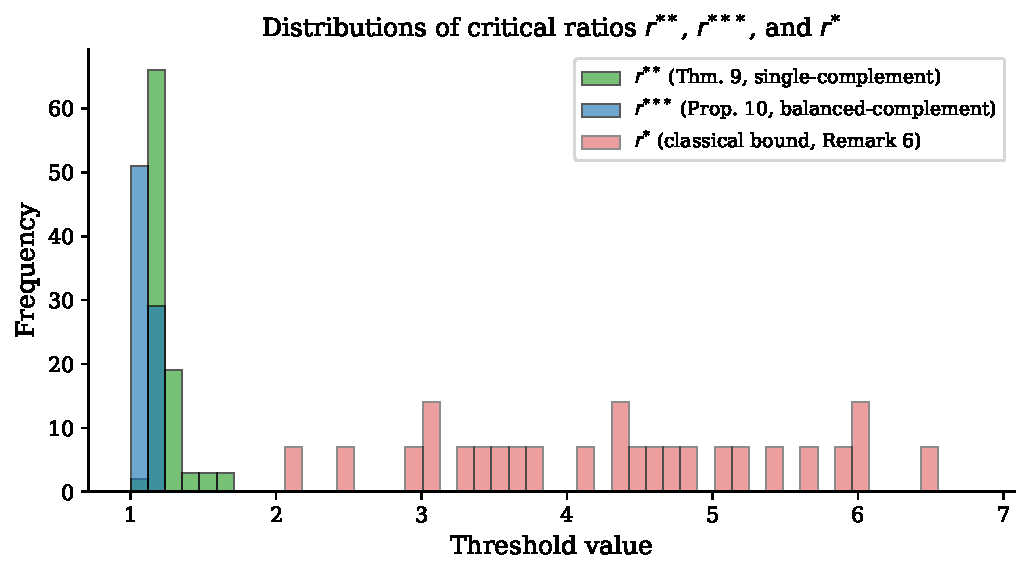
\includegraphics[width=0.8\textwidth]{fig5_rstar_vs_rss.pdf}
\caption{Histograms of $r^{\ast\ast}$, $r^{\ast\ast\ast}$, and $r^{\ast}$ over all NN instances. $r^{\ast\ast}$ and $r^{\ast\ast\ast}$ concentrate near the empirical $r$ (making them informative Core-emptiness thresholds via Corollary~\ref{cor:single-complement} and Corollary~\ref{cor:balanced-complement}); $r^{\ast}$ lies far to the right and rarely binds.}
\label{fig:rhist}
\end{figure}

\bibliographystyle{apalike-ejor}
\bibliography{references_ejor}

\end{document}
